%!TEX program = xelatex
\documentclass[11pt, a4paper]{article}

% AA LINGUA E GESTIONE FONT (Specifica per XeLaTeX)
\usepackage{fontspec}
\setmainfont{Latin Modern Roman}
\usepackage[italian]{babel}

% AA LAYOUT DI PAGINA E TIPOGRAFIA (Ottimizzato per Rilegatura)
\usepackage[left=2.4cm, right=1.6cm, top=2cm, bottom=2cm]{geometry}

% AA Spaziatura tra paragrafi controllata (compatta ed evita salti enormi)
\usepackage[skip=3pt plus 1pt minus 1pt]{parskip}
\setlength{\parindent}{0pt}

% AA Microtype per XeLaTeX
\usepackage[protrusion=true]{microtype}
\raggedbottom

% AA GESTIONE DEI COLORI
\usepackage{xcolor}

% AA MATEMATICA E SIMBOLI
\usepackage{amsmath}
\usepackage{mathtools}
\usepackage{silence}
\usepackage[warnings-off={mathtools-overbracket,mathtools-colon}]{unicode-math}
\setmathfont{Latin Modern Math}

% BB OTTIMIZZAZIONE MATRICI LUNGHE PER LA STAMPA
\setlength{\arraycolsep}{10pt}

% AA Spaziature verticali attorno alle formule matematiche
\setlength{\abovedisplayskip}{3pt plus 1pt minus 1pt}
\setlength{\belowdisplayskip}{3pt plus 1pt minus 1pt}
\setlength{\abovedisplayshortskip}{0pt plus 1pt}
\setlength{\belowdisplayshortskip}{2pt plus 1pt minus 1pt}

% AA GRAFICA ED IMMAGINI
\usepackage{graphicx}
\graphicspath{{./E9_Images/}}

% AA PERSONALIZZAZIONE TITOLI
\usepackage{titlesec}
\titleformat{\section}{\normalfont\Large\bfseries\color{blue!80!black}}{\thesection}{1em}{}
\titleformat{name=\section,numberless}{\normalfont\Large\bfseries\color{blue!80!black}}{}{0pt}{}

\titleformat{\subsection}{\normalfont\large\bfseries}{\thesubsection}{1em}{}
\titleformat{name=\subsection,numberless}{\normalfont\large\bfseries}{}{0pt}{}

\titleformat{\subsubsection}{\normalfont\normalsize\bfseries}{\thesubsubsection}{1em}{}
\titleformat{name=\subsubsection,numberless}{\normalfont\normalsize\bfseries}{}{0pt}{}

\titlespacing*{\section}{0pt}{1.2ex plus 0.4ex minus 0.2ex}{0.6ex plus 0.2ex}
\titlespacing*{\subsection}{0pt}{1ex plus 0.3ex minus 0.2ex}{0.5ex plus 0.2ex}
\titlespacing*{\subsubsection}{0pt}{0.8ex plus 0.2ex minus 0.1ex}{0.4ex plus 0.1ex}

\titleformat{\paragraph}[block]{\normalfont\normalsize\bfseries\color{black!80!black}\raggedright}{}{0pt}{}
\titlespacing*{\paragraph}{0pt}{1.2ex plus 0.3ex minus 0.2ex}{0.4ex}

% AA INTEGRAZIONE CODICE MATLAB
\usepackage{matlab}

% BB Riconfigurazione Automatica Titoli Esportati da MATLAB
\renewcommand{\matlabheading}[1]{\section*{#1}}
\renewcommand{\matlabheadingtwo}[1]{\subsection*{#1}}
\renewcommand{\matlabheadingthree}[1]{\subsubsection*{#1}}

% BB Formule E Matrici Simboliche
\renewenvironment{matlabsymbolicoutput}{%
  \par\vspace{2pt}%
  \begingroup
  \centering
}{%
  \par\vspace{2pt}%
  \endgroup
}

% BB Output Testuale Console
\renewenvironment{matlaboutput}{%
  \par\vspace{1pt}%
  \Verbatim[xleftmargin=10pt, formatcom=\color{black!75}, fontsize=\footnotesize]%
}{%
  \endVerbatim
  \vspace{1pt}%
}

% BB Box Codice (Stile Moderno con Barra Laterale Colorata)
\lstset{
  backgroundcolor={},
  aboveskip=0pt,
  belowskip=0pt,
  basicstyle=\ttfamily\footnotesize,
  xleftmargin=0pt
}

\mdfdefinestyle{matlabcode}{%
  topline=false,
  bottomline=false,
  rightline=false,
  leftline=true,
  linewidth=2.5pt,
  linecolor=blue!75!black,
  backgroundcolor=black!3,
  innertopmargin=4pt,
  innerbottommargin=4pt,
  innerleftmargin=9pt,
  innerrightmargin=6pt,
  skipabove=3pt,
  skipbelow=3pt
}

\allowdisplaybreaks

% AA LINK, METADATI ED ELENCHI
\usepackage{hyperref}
\hypersetup{
    colorlinks=true,
    linkcolor=blue!80!black,
    urlcolor=blue!80!black,
    citecolor=blue!80!black,
    pdftitle={Algoritmo Di Newton E Del Gradiente},
    pdfauthor={Francesco Lo Verde},
}
\usepackage{bookmark}

% BB Spaziatura Elenchi (Arieggiata per la Stampa)
\usepackage{enumitem}
\setlist{itemsep=3.5pt plus 1pt minus 1pt, topsep=4pt plus 1pt minus 1pt, partopsep=0pt, parsep=1pt}


\author{Francesco Lo Verde}
\begin{document}

\label{T_9c72}
\matlabtitle{Implementazione Algoritmo Di Newton E Del Gradiente}

\begin{par}
\begin{flushleft}
La prima fase consiste nella definizione del modello cinematico del manipolatore. Si utilizzano variabili simboliche per rappresentare le lunghezze dei bracci e le variabili di giunto, al fine di ottenere espressioni generali e analitiche.
\end{flushleft}
\end{par}

\begin{matlabcode}
clc; clear; close all;
% Variabili Di Giunto
syms q1 q2 real;

% Lunghezza Bracci
syms l1 l2 real;
\end{matlabcode}

\begin{par}
\begin{center}
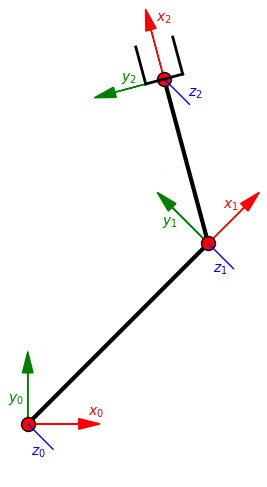
\includegraphics[width=0.3\linewidth]{figure_2}
\end{center}
\end{par}

\begin{matlabcode}
% Posizione Base Giunto
x0 = 0;
y0 = 0;

% Calcolo Coordinate Fine Primo Braccio (x1, y1)
x1 = l1 * cos(q1);
y1 = l1 * sin(q1);

% Calcolo Coordinate End Effector (x2, y2) Rispetto Al Sistema Di Riferimento Base
x = x1 + l2 * cos(q1 + q2);
y = y1 + l2 * sin(q1 + q2);

% Definizione Vettore Colonna fr_q = [x; y]
fr_q = [x; y];
fr_q = simplify(fr_q);

% Definizione Vettore Variabili Di Giunto
q = [q1; q2];

fprintf('Posizione EE Rispetto Al Riferimento Base [Vettore fr(q)]');
disp(fr_q);
\end{matlabcode}
\begin{matlaboutput}
Posizione EE Rispetto Al Riferimento Base [Vettore fr(q)]
\end{matlaboutput}
\begin{matlabsymbolicoutput}
\hskip1em $\displaystyle \left(\begin{array}{c}
l_2 \,\cos \left(q_1 +q_2 \right)+l_1 \,\cos \left(q_1 \right)\\
l_2 \,\sin \left(q_1 +q_2 \right)+l_1 \,\sin \left(q_1 \right)
\end{array}\right)$
\end{matlabsymbolicoutput}
\newpage
\begin{par}
\begin{flushleft}
Per sviluppare gli algoritmi di cinematica inversa, è fondamentale calcolare la matrice Jacobiana, che lega le velocità nello spazio dei giunti alle velocità nello spazio operativo.
\end{flushleft}
\end{par}

\begin{matlabcode}
% Calcolo Jacobiano Analitico
J_q = jacobian(fr_q, q);
J_q = simplify(J_q);
fprintf('\nJacobiano Analitico J(q):\n');
\end{matlabcode}
\begin{matlaboutput}
Jacobiano Analitico J(q):
\end{matlaboutput}
\begin{matlabcode}
disp(J_q);
\end{matlabcode}
\begin{matlabsymbolicoutput}
\hskip1em $\displaystyle \left(\begin{array}{cc}
-l_2 \,\sin \left(q_1 +q_2 \right)-l_1 \,\sin \left(q_1 \right) & -l_2 \,\sin \left(q_1 +q_2 \right)\\
l_2 \,\cos \left(q_1 +q_2 \right)+l_1 \,\cos \left(q_1 \right) & l_2 \,\cos \left(q_1 +q_2 \right)
\end{array}\right)$
\end{matlabsymbolicoutput}
\begin{matlabcode}

% Definizione simbolica della Posa Desiderata
syms rx ry real;
r = [rx; ry];
\end{matlabcode}

\begin{par}
\begin{flushleft}
Data la funzione di cinematica diretta $f_r (q)$, che mappa lo spazio dei giunti allo spazio operativo, si vuole trovare $q$ tale che $f_r (q)=r$. Per risolvere questo problema numericamente, si definisce un vettore di errore $e$ che quantifica la "distanza" tra la posa desiderata $r$ e quella attuale $f_r (q)$:
\end{flushleft}
\end{par}

\label{H_2276}
\matlabheadingthree{$e(q)\triangleq r-f_r (q)$}

\begin{par}
\begin{flushleft}
L'obiettivo è far convergere questo errore a zero.
\end{flushleft}
\end{par}

\begin{matlabcode}
% Definizione Vettore Di Errore e(q) = r - fr(q)
e_q = r - fr_q;

% Definizione Funzione Di Costo Scalare V(q) (Norma Dell'Errore Al Quadrato)
% V = (1/2) * e^T * e, che in MATLAB si traduce in e' * e
V = (1/2) * (e_q.' * e_q);
V = simplify(V);

fprintf('\nFunzione Di Costo V(q):\n');
disp(V);
\end{matlabcode}
\begin{matlaboutput}
Funzione Di Costo V(q):
\end{matlaboutput}
\begin{matlabsymbolicoutput}
\hskip1em $\displaystyle \frac{{{\left(l_2 \,\cos \left(q_1 +q_2 \right)-\textrm{rx}+l_1 \,\cos \left(q_1 \right)\right)}}^2 }{2}+\frac{{{\left(l_2 \,\sin \left(q_1 +q_2 \right)-\textrm{ry}+l_1 \,\sin \left(q_1 \right)\right)}}^2 }{2}$
\end{matlabsymbolicoutput}

\begin{par}
\begin{flushleft}
Per analizzare il comportamento della funzione di costo $V(q)$, è necessario studiarne i punti stazionari. Questi si trovano dove il gradiente della funzione è nullo. La natura di tali punti (minimi, massimi, selle) è determinata dalla matrice Hessiana.
\end{flushleft}
\end{par}

\begin{par}
\begin{flushleft}
La Matrice Hessiana di una funzione scalare V è la Jacobiana del suo gradiente, cioè
\end{flushleft}
\end{par}

\label{H_47da}
\matlabheadingthree{ $H_V =\frac{d(\nabla_q V)}{dq}$ }

\begin{par}
$H_V (q)=J(q)^T J(q)-\sum_{k=1}^m e_k (q)H_{f_k } (q)$
\end{par}

\begin{matlabcode}
% Calcolo Gradiente V(q)
gradV = -J_q.' * e_q;
gradV = simplify(gradV);

% Calcolo Matrice Hessiana
% H_V(i,j) = d^2(V) / (dq_i * dq_j)
H_V = hessian(V, q);
H_V = simplify(H_V);
\end{matlabcode}
\newpage
\begin{matlabcode}
fprintf('Matrice Hessiana:');
disp(H_V);
\end{matlabcode}
\begin{matlaboutput}
Matrice Hessiana:
\end{matlaboutput}
\begin{matlabsymbolicoutput}
\resizebox{\linewidth}{!}{%
$
\begin{pmatrix}
    l_1 \,\textrm{rx}\,\cos \left(q_1 \right)+l_1 \,\textrm{ry}\,\sin \left(q_1 \right)+l_2 \,\textrm{rx}\,\cos \left(q_1 +q_2 \right)+l_2 \,\textrm{ry}\,\sin \left(q_1 +q_2 \right) & \sigma_1 \\
    \sigma_1  & l_2 \,{\left(\textrm{rx}\,\cos \left(q_1 +q_2 \right)+\textrm{ry}\,\sin \left(q_1 +q_2 \right)-l_1 \,\cos \left(q_2 \right)\right)}
\end{pmatrix}
$%
}

\vspace{0.5em}
\noindent Dove:
\vspace{-0.5em}

\[
\begin{aligned}
\;\;\sigma_1 =l_2 \,\textrm{rx}\,\cos \left(q_1 +q_2 \right)+l_2 \,\textrm{ry}\,\sin \left(q_1 +q_2 \right)
\end{aligned}
\]
\end{matlabsymbolicoutput}
\begin{matlabcode}
% Calcolo Jacobiana Gradiente Di V
%H_V_Da_Grad = jacobian(gradV, q);
\end{matlabcode}

\begin{par}
\begin{flushleft}
I punti critici si trovano risolvendo l'equazione precedente $\nabla_q V=0$.  La loro classificazione dipende dagli autovalori della matrice Hessiana $H_V$ valutata in tali punti:
\end{flushleft}
\end{par}

\begin{itemize}
   \item{\begin{flushleft} \textbf{Minimo Locale: }Hessiana definita positiva (autovalori tutti positivi) \end{flushleft}}
   \item{\begin{flushleft} \textbf{Massimo Locale: }Hessiana definita negativa (autovalori tutti negativi) \end{flushleft}}
   \item{\begin{flushleft} \textbf{Punto Sella: }Hessiana indefinita (autovalori di segno discordi) \end{flushleft}}
\end{itemize}

\newpage
\matlabheadingtwo{Algoritmo Di Newton}

\begin{par}
\begin{flushleft}
L'idea alla base del metodo di Newton, in questo contesto, è di trattare il problema come un sistema di controllo in cui si progetta una velocità dei giunti $\dot{q}$ per annullare l'errore.
\end{flushleft}
\end{par}

\begin{par}
\begin{flushleft}
L'algoritmo iterativo deve fornire un evoluzione per $\underline{q}$ tale che $q\to \underline{q}$ in modo che
\end{flushleft}
\end{par}

\label{H_7088}
\matlabheadingthree{$\dot{e} \bigl(\underline{q} \bigr)=\dot{r} -f_r \bigl(\underline{q} \bigr)=\dot{r} -J_r \bigl(\underline{q} \bigr)\;\dot{q}$}

\begin{par}
\begin{flushleft}
Si consideri la matrice $J$ quadrata e non singolare e imponendo
\end{flushleft}
\end{par}

\label{H_9ab9}
\matlabheadingthree{$\dot{e} =K\cdot e$}

\begin{par}
\begin{flushleft}
Quando gli autovalori di $K$ sono tutti a parte reale negativa si fa tendere l'errore a \textit{\textbf{zero}}\textit{. }Quindi
\end{flushleft}
\end{par}

\label{H_29de}
\matlabheadingthree{$\dot{r} -J_r \bigl(\underline{q} \bigr)\;\dot{q} =K\cdot e$}

\begin{par}
\begin{flushleft}
Da cui si può ottenere $\dot{q}$ come:
\end{flushleft}
\end{par}

\label{H_351f}
\matlabheadingthree{$\dot{q} =J_r^{-1} \bigl(\underline{q} \bigr)\;\bigl\lbrack \dot{r} -K\cdot e\bigr\rbrack$}

\begin{par}
\begin{flushleft}
La legge di controllo per l'algoritmo di Newton viene derivata imponendo una convergenza esponenziale all'errore, $\dot{e} =K\cdot e$ dove $K$ è una matrice i cui autovalori hanno parte reale negativa per garantire la stabilità. Partendo dalla relazione cinematica $\dot{e} =\dot{r} -J(q)\cdot \dot{q}$ si ottiene:
\end{flushleft}
\end{par}

\label{H_29c9}
\matlabheadingthree{$\dot{r} -J(q)\cdot \dot{q} =K\cdot e$}

\begin{par}
\begin{flushleft}
Da cui:
\end{flushleft}
\end{par}

\label{H_9626}
\matlabheadingthree{$J(q)\cdot \dot{q} =\dot{r} -K\cdot e$}

\begin{par}
\begin{flushleft}
La risoluzione di questa equazione per $\dot{q}$ dipende dalla natura della matrice Jacobiana $J(q)$.
\end{flushleft}
\end{par}

\begin{par}
\begin{flushleft}
\textbf{Caso Non Quadrato:} Se il numero di giunti $n$ è maggiore dei gradi di libertà del task $m$, la Jacobiana non è quadrata e non è invertibile. Si ricorre alla pseudoinversa $J\#$ per trovare una soluzione. La formula generale è:
\end{flushleft}
\end{par}

\label{H_4e5b}
\matlabheadingthree{$\dot{q} =J\# (q)\cdot \bigl\lbrack \dot{r} -K\cdot e\bigr\rbrack +\bigl(I-J\# (q)J(q)\bigr)\cdot {\dot{q} }_0$}

\begin{enumerate}
\setlength{\itemsep}{-1ex}
   \item{\begin{flushleft} Il primo termine della somma calcola la soluzione per $\dot{q}$ a norma minima che esegue il compito di raggiungere $r$. \end{flushleft}}
   \item{\begin{flushleft} Il secondo termine della somma proietta una velocità di giunto arbitraria ${\dot{q} }_0$ nello spazio nullo della Jacobiana (\textbf{movimenti interni}).  \end{flushleft}}
\end{enumerate}

\begin{par}
\begin{flushleft}
Questo permette di gestire compiti secondari senza influenzare il movimento dell'end-effector. Per il manipolatore RR planare, questo caso non si applica poiché $n=m=2$.
\end{flushleft}
\end{par}

\begin{par}
\begin{flushleft}
\textbf{Caso Quadrato E Non Singolare:} La Jacobiana è una matrice 2x2. Se non è singolare, la pseudoinversa coincide con l'inversa classica ($J\# =J^{-1}$) e il termine dello spazio nullo  si annulla ($I-J^{-1} (q)J(q)=0$). La formula si semplifica notevolmente in:
\end{flushleft}
\end{par}

\label{H_28f6}
\matlabheadingthree{$\dot{q} =J^{-1} (q)\cdot \bigl\lbrack \dot{r} -K\cdot e\bigr\rbrack$}

\newpage
\begin{par}
\begin{flushleft}
L' obiettivo è raggiungere una \textit{\textbf{posa fissa}}, quindi la velocità desiderata dell'end-effector è nulla per tutto il tempo.
\end{flushleft}
\end{par}

\begin{matlabcode}
syms q1_dot q2_dot real;
q_dot = [q1_dot; q2_dot];

% Assumendo \dot{r} Costante

% Calcolo Derivata Errore
% e = \dot{r} - J_{r}\bigl(\underline{q} \bigr) \; \dot{q}
e_dot = -J_q * q_dot;

fprintf('Relazione Tra Derivata Errore E Velocità Giunti:');
\end{matlabcode}
\begin{matlaboutput}
Relazione Tra Derivata Errore E Velocità Giunti:
\end{matlaboutput}
\begin{matlabcode}
disp(e_dot);
\end{matlabcode}
\begin{matlabsymbolicoutput}
\hskip1em $\displaystyle \left(\begin{array}{c}
q_{\dot{1} } \,{\left(l_2 \,\sin \left(q_1 +q_2 \right)+l_1 \,\sin \left(q_1 \right)\right)}+l_2 \,q_{\dot{2} } \,\sin \left(q_1 +q_2 \right)\\
-q_{\dot{1} } \,{\left(l_2 \,\cos \left(q_1 +q_2 \right)+l_1 \,\cos \left(q_1 \right)\right)}-l_2 \,q_{\dot{2} } \,\cos \left(q_1 +q_2 \right)
\end{array}\right)$
\end{matlabsymbolicoutput}
\begin{matlabcode}

% Definizione Matrice Guadagno Esponenziale
% Scelta Comune: Matrice Diagonale I
syms k real;
K = k * eye(2);

e_dot_Target = - K * e_q;
fprintf("Errore Desiderato (Target):");
\end{matlabcode}
\begin{matlaboutput}
Errore Desiderato (Target):
\end{matlaboutput}
\begin{matlabcode}
disp(e_dot_Target);
\end{matlabcode}
\begin{matlabsymbolicoutput}
\hskip1em $\displaystyle \left(\begin{array}{c}
k\,{\left(l_2 \,\cos \left(q_1 +q_2 \right)-\textrm{rx}+l_1 \,\cos \left(q_1 \right)\right)}\\
k\,{\left(l_2 \,\sin \left(q_1 +q_2 \right)-\textrm{ry}+l_1 \,\sin \left(q_1 \right)\right)}
\end{array}\right)$
\end{matlabsymbolicoutput}
\begin{matlabcode}

% Risoluzione Per Velocità Giunto
eqPerDotq = e_dot == e_dot_Target;

q_dot_eq = inv(J_q) * (K * e_q);
q_dot_eq = simplify(q_dot_eq);
fprintf("Equazione Di q_dot (Velocità Giunti)");
\end{matlabcode}
\begin{matlaboutput}
Equazione Di q_dot (Velocità Giunti)
\end{matlaboutput}
\begin{matlabcode}
disp(q_dot_eq);
\end{matlabcode}
\begin{matlabsymbolicoutput}
\hskip1em $\displaystyle \left(\begin{array}{c}
-\frac{k\,{\left(l_2 -\textrm{rx}\,\cos \left(q_1 +q_2 \right)-\textrm{ry}\,\sin \left(q_1 +q_2 \right)+l_1 \,\cos \left(q_2 \right)\right)}}{l_1 \,\sin \left(q_2 \right)}\\
-\frac{k\,{\left(l_1 \,\textrm{rx}\,\cos \left(q_1 \right)-{l_2 }^2 -2\,l_1 \,l_2 \,\cos \left(q_2 \right)-{l_1 }^2 +l_1 \,\textrm{ry}\,\sin \left(q_1 \right)+l_2 \,\textrm{rx}\,\cos \left(q_1 +q_2 \right)+l_2 \,\textrm{ry}\,\sin \left(q_1 +q_2 \right)\right)}}{l_1 \,l_2 \,\sin \left(q_2 \right)}
\end{array}\right)$
\end{matlabsymbolicoutput}


\vspace{1em}
\begin{par}
\begin{flushleft}
Per implementare questo metodo si deve discretizzare la legge di controllo. Utilizzando il metodo di Eulero con un passo di campionamento $T$, assumento $\dot{r} =0$ e includendo il meno nella matrice $K$ l'aggiornamento della posizione dei giunti diventa:
\end{flushleft}
\end{par}

\label{H_1dd8}
\matlabheadingthree{$q_{k+1} =q_k +T\cdot J^{-1} (q_k )\cdot \bigl\lbrack K\cdot e(k)\bigr\rbrack$}

\newpage
\matlabheadingthree{\textbf{Algoritmo Del Gradiente}}

\begin{par}
\begin{flushleft}
Un approccio alternativo al metodo di Newton consiste nel riformulare il problema come uno di \textbf{ottimizzazione}. L'obiettivo non è più risolvere un sistema di equazioni (trovare gli zeri di $e(q)$), ma minimizzare una funzione di costo, che in questo caso è la norma quadratica dell'errore $V(q)$.
\end{flushleft}
\end{par}

\begin{par}
\begin{flushleft}
Per garantire che $V(q)$ diminuisca, la sua derivata temporale, $\dot{V}$, deve essere negativa. Applicando la regola della catena e la relazione cinematica $\dot{e} =-J(q)\dot{q}$ (assumendo $\dot{r} =0$), si ottiene:
\end{flushleft}
\end{par}

\label{H_46dd}
\matlabheadingthree{$\dot{V} =e^T \dot{e} =-e^T J(q)\;\dot{q}$}

\begin{par}
\begin{flushleft}
Una scelta intuitiva per $\dot{q}$ che garantisce $\dot{V} \le 0$ è la \textit{\textbf{legge del gradiente}}, che muove i giunti nella direzione opposta a quella del gradiente della funzione di costo ($\nabla_q V=-J(q)^T e$):
\end{flushleft}
\end{par}

\label{H_0d42}
\matlabheadingthree{$\dot{q} =\alpha \cdot J(q)^T e(q)$}

\begin{par}
\begin{flushleft}
dove $\alpha >0$ è un guadagno scalare positivo (\textbf{learning rate}). Sostituendo questa legge in $\dot{V}$, si verifica la stabilità:
\end{flushleft}
\end{par}

\label{H_9194}
\matlabheadingthree{$\dot{V} =-e^T J(q)\;(\alpha J(q)^T e)=-\alpha (J(q)^T e)^T (J(q)^T e)=-\alpha \|J(q)^T e{\|}^2 \le 0$}

\begin{par}
\begin{flushleft}
L'algoritmo si arresta quando $\dot{V} =0$, il che accade quando si raggiunge un punto critico $\nabla_q V=0$.
\end{flushleft}
\end{par}

\begin{matlabcode}
% Definizione Learning Rate
syms alpha

% Velocità Dei Giunti
q_dot_grad = alpha * J_q.' * e_q;
q_dot_grad = simplify(q_dot_grad);

fprintf('Equazione Velocità Dei Giunti:');
\end{matlabcode}
\begin{matlaboutput}
Equazione Velocità Dei Giunti:
\end{matlaboutput}
\begin{matlabcode}
disp(q_dot_grad);
\end{matlabcode}
\begin{matlabsymbolicoutput}
\hskip1em $\displaystyle \left(\begin{array}{c}
\alpha \,{\left(l_1 \,\textrm{ry}\,\cos \left(q_1 \right)-l_1 \,\textrm{rx}\,\sin \left(q_1 \right)+l_2 \,\textrm{ry}\,\cos \left(q_1 +q_2 \right)-l_2 \,\textrm{rx}\,\sin \left(q_1 +q_2 \right)\right)}\\
\alpha \,l_2 \,{\left(\textrm{ry}\,\cos \left(q_1 +q_2 \right)-\textrm{rx}\,\sin \left(q_1 +q_2 \right)+l_1 \,\sin \left(q_2 \right)\right)}
\end{array}\right)$
\end{matlabsymbolicoutput}

\begin{par}
\begin{flushleft}
L'analisi della funzione di costo $V(q)$ è fondamentale per comprendere il comportamento degli algoritmi di ottimizzazione, in particolare quello del gradiente. I punti critici (o \textit{stazionari}) si trovano dove il gradiente di $V(q)$ si annulla, ovvero $\nabla_q V=-J(q)^T e(q)=0$. Questi punti non corrispondono necessariamente alla soluzione desiderata ($e=0$), ma possono rappresentare minimi locali o punti di sella in cui l'algoritmo del gradiente può arrestarsi prematuramente.
\end{flushleft}
\end{par}

\begin{par}
\begin{flushleft}
Per classificare un punto critico $q_c$ (per cui $\nabla_q V(q_c )=0$), si analizzano gli autovalori della matrice Hessiana $H_V (q_c )$ valutata in quel punto:
\end{flushleft}
\end{par}

\begin{itemize}
\setlength{\itemsep}{-1ex}
   \item{\begin{flushleft} \textbf{Minimo Locale: }Hessiana definita positiva (autovalori tutti positivi) \end{flushleft}}
   \item{\begin{flushleft} \textbf{Massimo Locale: }Hessiana definita negativa (autovalori tutti negativi) \end{flushleft}}
   \item{\begin{flushleft} \textbf{Punto Sella: }Hessiana indefinita (autovalori di segno discordi) \end{flushleft}}
\end{itemize}


\newpage
\matlabheadingtwo{Analisi Massimi E Punti Sella Funzione “Norma Errore Al Quadrato"}

\begin{par}
\begin{flushleft}
Le espressioni simboliche derivate in precedenza vengono rese numeriche assegnando valori numerici alle lunghezze dei bracci (\texttt{l1}, \texttt{l2}) e alla posa desiderata dell'end-effector (\texttt{r}). Questo permette di calcolare le posizioni numeriche dei punti critici, e classificare esplicitamente i punti critici calcolando gli autovalori della matrice Hessiana.
\end{flushleft}
\end{par}

\begin{matlabcode}

% Definizione Parametri Numerici Manipolatore
l_val = [1, 0.8];
r_val = [1.3, 0.5];

% Sostituzione Simbolica
% V, gradV, H_V Già Calcolati
% V = (1/2) * (e_q.' * e_q);
V_val = subs(V, [l1, l2, rx, ry], [l_val(1), l_val(2), r_val(1), r_val(2)]);
gradV_val = subs(gradV, [l1, l2, rx, ry], [l_val(1), l_val(2), r_val(1), r_val(2)]);
H_V_val = subs(H_V, [l1, l2, rx, ry], [l_val(1), l_val(2), r_val(1), r_val(2)]);
\end{matlabcode}

\begin{par}
\begin{flushleft}
Una volta ottenuta l'espressione numerica del gradiente, il passo successivo consiste nell'identificare i punti stazionari della funzione di costo. Tali punti, per definizione, sono le configurazioni \texttt{q} in cui il gradiente si annulla, ovvero
\end{flushleft}
\end{par}

\begin{par}
$\nabla_q V=-J(q)^T e(q)=0$
\end{par}

\begin{par}
\begin{flushleft}
La risoluzione di questo sistema di equazioni permette di individuare tutte le configurazioni del manipolatore che sono candidate a essere minimi, massimi o punti di sella per la funzione di errore.
\end{flushleft}
\end{par}

\begin{matlabcode}
% Calcolo Punti Critici
[q1Staz, q2Staz, param, conditions] = solve(gradV_val == [0;0], [q1, q2], "ReturnConditions",true, 'Real',true);

fprintf('Valori q_1:');
disp(q1Staz);
\end{matlabcode}
\begin{matlaboutput}
Valori q_1:
\end{matlaboutput}

\begin{matlabsymbolicoutput}
\hskip1em $\displaystyle \left(\begin{array}{c}
2\,\textrm{atan}\left(\frac{\sqrt{247}}{49}+\frac{10}{49}\right)+2\,\pi \,l\\
2\,\pi \,l-2\,\textrm{atan}\left(\frac{\sqrt{247}}{49}-\frac{10}{49}\right)\\
\textrm{atan}\left(\frac{5}{13}\right)-\pi +2\,\pi \,l\\
2\,\textrm{atan}\left(\frac{\sqrt{194}}{5}-\frac{13}{5}\right)+2\,\pi \,l\\
2\,\pi \,l-2\,\textrm{atan}\left(\frac{\sqrt{194}}{5}+\frac{13}{5}\right)\\
\textrm{atan}\left(\frac{5}{13}\right)+2\,\pi \,l
\end{array}\right)$
\end{matlabsymbolicoutput}
\begin{matlabcode}
fprintf('Valori q_2:');
disp(q2Staz);
\end{matlabcode}
\begin{matlaboutput}
Valori q_2:
\end{matlaboutput}
\begin{matlabsymbolicoutput}
\hskip1em $\displaystyle \left(\begin{array}{c}
2\,\pi \,m-2\,\textrm{atan}\left(\frac{\sqrt{247}}{19}\right)\\
2\,\textrm{atan}\left(\frac{\sqrt{247}}{19}\right)+2\,\pi \,m\\
-\pi \,{\left(2\,m-1\right)}\\
2\,\pi \,m\\
2\,\pi \,m\\
-\pi \,{\left(2\,m-1\right)}
\end{array}\right)$
\end{matlabsymbolicoutput}
\begin{matlabcode}
fprintf('Condizione: ');
disp(conditions(1));
\end{matlabcode}
\begin{matlaboutput}
Condizione:
\end{matlaboutput}
\begin{matlabsymbolicoutput}
\hskip1em $\displaystyle l\in \mathbb{Z}\wedge m\in \mathbb{Z}$
\end{matlabsymbolicoutput}

\begin{par}
\begin{flushleft}
I vettori \texttt{q1Staz} e \texttt{q2Staz} contengono le espressioni generali per le soluzioni. I parametri \texttt{\textit{l}}\textit{ }e\textit{ }\texttt{\textit{m }}rappresentano multipli interi di rotazioni complete ($2\pi$) e le condizioni definiscono il dominio dei parametri. In sintesi:
\end{flushleft}
\end{par}

\begin{par}
\begin{flushleft}
\textbf{Le soluzioni per }$(q_1 ,q_2 )$\textbf{ sono quelle descritte dalle formule in }\texttt{\textbf{q1Staz}}\textbf{ e }\texttt{\textbf{q2Staz}}\textbf{, a condizione che }\texttt{\textit{\textbf{l}}}\textit{\textbf{ }}\textbf{e}\textit{\textbf{ }}\texttt{\textit{\textbf{m}}}\textbf{ siano numeri interi.}
\end{flushleft}
\end{par}

\begin{par}
\begin{flushleft}
Per quanto riguarda il manipolatore RR planare, questo risultato significa che ci sono diversi modi per raggiungere i punti critici della funzione di errore. Si consideramp le \textbf{configurazioni fisiche uniche}. Ad esempio, una configurazione $(q_1 ,q_2 )=\biggl(\frac{\pi }{2},0\biggr)$ è identica a $(q_1 ,q_2 )=\biggl(\frac{\pi }{2}+2\pi ,0\biggr)$. Per l'analisi, è sufficiente considerare solo le soluzioni comprese nell'intervallo $[-\pi ,\pi ]$.
\end{flushleft}
\end{par}

\begin{par}
\begin{flushleft}
Le soluzioni simboliche devono essere convertite in un insieme finito di punti numerici per poter procedere con l'analisi. Si effettua una ricerca sistematica assegnando ad \texttt{\textit{l }}e \texttt{\textit{m}}\texttt{ }un range di valori interi e per ogni coppia $(l,m)$, si calcolano i valori numerici. Successivamente, vengono scartate le soluzioni che non sono nell'intervallo $[-\pi ,\pi ]$ ed eventuali duplicati.
\end{flushleft}
\end{par}

\begin{matlabcode}
% Matrice Punti Critici
% Ogni Riga È (q1, q2)
puntiCritici = [];

for i = 1:length(q1Staz)
    for l_test = -2:2
        for m_test = -2:2

            % pCritic = double(subs([q1Staz(i); q2Staz(i)], [l, m], [l_val, m_val]));
            pCritic = subs([q1Staz(i); q2Staz(i)], [param(1), param(2)], [l_test, m_test]);

            puntiCritici = [puntiCritici; pCritic.'];

        end
    end
end

% Normalizzazione e Rimozione dei Duplicati
% Il modo più robusto per normalizzare è atan2(sin(q), cos(q))
puntiCritici = atan2(sin(puntiCritici), cos(puntiCritici));
puntiCritici = double(puntiCritici);

\end{matlabcode}
\newpage
\begin{matlabcode}
% uniquetol Estrae Valori Unici
puntiCritici = uniquetol(puntiCritici, 1e-6, 'ByRows', true);

fprintf('Punti Critici (q1, q2) In Radianti:\n');
disp(puntiCritici);
\end{matlabcode}

\begin{matlaboutput}
Punti Critici (q1, q2) In Radianti:
   -2.7744         0
   -2.7744    3.1416
   -0.2323    1.3822
    0.3672         0
    0.3672    3.1416
    0.9666   -1.3822
\end{matlaboutput}

\begin{par}
\begin{flushleft}
Dopo aver calcolato l'insieme dei punti critici unici, il passo successivo consiste nella loro classificazione. Come detto prima si analizzano gli autovalori della matrice Hessiana $H_V (q_c )$ valutata in quel punto.
\end{flushleft}
\end{par}

\begin{matlabcode}
fprintf('Matrice Hessiana H_V(q):')
\end{matlabcode}
\begin{matlaboutput}
Matrice Hessiana H_V(q):
\end{matlaboutput}
\begin{matlabcode}
disp(H_V_val);
\end{matlabcode}
\begin{matlabsymbolicoutput}
\[
\begin{pmatrix}
    \sigma_2 +\sigma_1 +\dfrac{13\,\cos \left(q_1 \right)}{10}+\dfrac{\sin \left(q_1 \right)}{2} & \sigma_2 +\sigma_1 \\[8pt]
    \sigma_2 +\sigma_1  & \sigma_2 +\sigma_1 -\dfrac{4\,\cos \left(q_2 \right)}{5}
\end{pmatrix}
\]

\vspace{0.5em}
\noindent\text{where}
\vspace{-0.5em}

\[
\begin{aligned}
    \sigma_1 &= \frac{2\,\sin \left(q_1 +q_2 \right)}{5} \\[4pt]
    \sigma_2 &= \frac{26\,\cos \left(q_1 +q_2 \right)}{25}
\end{aligned}
\]
\end{matlabsymbolicoutput}
\begin{matlabcode}
for i = 1:size(puntiCritici, 1)
    q1Crit = puntiCritici(i,1);
    q2Crit = puntiCritici(i,2);
    fprintf('Configurazione Critica (q1, q2) = (%.4f, %.4f)\n', q1Crit, q2Crit);

    H_V_Current = subs(H_V_val, [q1, q2], [q1Crit, q2Crit]);
    H_V_Current = double(H_V_Current);
    % disp(H_V_Current);

    lambda = eig(H_V_Current);
    fprintf('\t Autovalori:\n');
    fprintf('\t %.4f\n', lambda);

    % Calcolo Errore
    rx_val = r_val(1);
    ry_val = r_val(2);
    l1_val = l_val(1);
    l2_val = l_val(2);

    e_q_val = subs(e_q, [rx, ry, l1, l2, q1, q2], [rx_val, ry_val, l1_val, l2_val, q1Crit, q2Crit]);
    e_q_val = double(e_q_val);
    norm_e_q = norm(e_q_val);
\end{matlabcode}
\newpage
\begin{matlabcode}
    fprintf('\t Vettore Errore e = r - fr_q:\n');
    fprintf('\t %.4f\n', e_q_val);
    fprintf('\t Norma Vettore Errore ||e||: %.4f\n', norm_e_q);
    if all(lambda > 0)
        % Hessiana Definita Positiva -> Minimo
        if norm_e_q < 1e-6
            fprintf('\t (%.4f, %.4f) È Minimo Globale\n', q1Crit, q2Crit);
        else
            fprintf('\t (%.4f, %.4f) È Minimo Locale\n', q1Crit, q2Crit);
        end
    elseif all(lambda < 0)
        % Hessiana Definita Positiva -> Massimo
        fprintf('\t (%.4f, %.4f) È Massimo Locale\n', q1Crit, q2Crit);
    else
        % L'Hessiana è indefinita -> Punto di Sella
        fprintf('\t (%.4f, %.4f) È Punto di Sella\n', q1Crit, q2Crit);
    end
end
\end{matlabcode}
\begin{matlaboutput}
Configurazione Critica (q1, q2) = (-2.7744, 0.0000)
	 Autovalori:
	 -3.3637
	 -1.0577
	 Vettore Errore e = r - fr_q:
	 2.9800
	 1.1462
	 Norma Vettore Errore ||e||: 3.1928
	 (-2.7744, 0.0000) È Massimo Locale
Configurazione Critica (q1, q2) = (-2.7744, 3.1416)
	 Autovalori:
	 -0.7454
	 2.3811
	 Vettore Errore e = r - fr_q:
	 1.4867
	 0.5718
	 Norma Vettore Errore ||e||: 1.5928
	 (-2.7744, 3.1416) È Punto di Sella
Configurazione Critica (q1, q2) = (-0.2323, 1.3822)
	 Autovalori:
	 0.2670
	 2.3130
	 Vettore Errore e = r - fr_q:
	 0.0000
	 -0.0000
	 Norma Vettore Errore ||e||: 0.0000
	 (-0.2323, 1.3822) È Minimo Globale
Configurazione Critica (q1, q2) = (0.3672, 0.0000)
	 Autovalori:
	 -0.1526
	 2.9739
	 Vettore Errore e = r - fr_q:
	 -0.3800
	 -0.1462
	 Norma Vettore Errore ||e||: 0.4072
	 (0.3672, 0.0000) È Punto di Sella
\end{matlaboutput}
\newpage
\begin{matlaboutput}
Configurazione Critica (q1, q2) = (0.3672, 3.1416)
	 Autovalori:
	 -1.1709
	 1.1352
	 Vettore Errore e = r - fr_q:
	 1.1133
	 0.4282
	 Norma Vettore Errore ||e||: 1.1928
	 (0.3672, 3.1416) È Punto di Sella
Configurazione Critica (q1, q2) = (0.9666, -1.3822)
	 Autovalori:
	 0.2670
	 2.3130
	 Vettore Errore e = r - fr_q:
	 0.0000
	 0.0000
	 Norma Vettore Errore ||e||: 0.0000
	 (0.9666, -1.3822) È Minimo Globale
\end{matlaboutput}


\vspace{1em}
\begin{matlabcode}
% Caricamento Immagini
img1 = imread('./Immagini/Singolarita1.png');
img2 = imread('./Immagini/Singolarita2.png');
img3 = imread('./Immagini/Singolarita3.png');
img4 = imread('./Immagini/Singolarita4.png');
img5 = imread('./Immagini/Singolarita5.png');
img6 = imread('./Immagini/Singolarita6.png');

% Figura
figure('Units','normalized','Position',[0 0 1 1]);
% Layout 5 Righe x 2 Colonne
t = tiledlayout(5,2,'TileSpacing','none','Padding','none');

% Riga 1
nexttile;
imshow(img1);
axis image off
title(sprintf('Singolarità 1 (%.4f, %.4f)', puntiCritici(1,1), puntiCritici(1,2)),'FontSize',14);

nexttile;
imshow(img2);
axis image off
title(sprintf('Singolarità 2 (%.4f, %.4f)', puntiCritici(2,1), puntiCritici(2,2)),'FontSize',14);

% Riga 2 Vuota
ax = nexttile([1 2]);
axis(ax,'off');

% Riga 3
nexttile;
imshow(img3);
axis image off
title(sprintf('Singolarità 3 (%.4f, %.4f)', puntiCritici(3,1), puntiCritici(3,2)),'FontSize',14);

nexttile;
imshow(img4);
axis image off
title(sprintf('Singolarità 4 (%.4f, %.4f)', puntiCritici(4,1), puntiCritici(4,2)),'FontSize',14);
\end{matlabcode}
\newpage
\begin{matlabcode}
% Riga 4 Vuota
ax = nexttile([1 2]);
axis(ax,'off');

% Riga 5
nexttile;
imshow(img5);
axis image off
title(sprintf('Singolarità 5 (%.4f, %.4f)', puntiCritici(5,1), puntiCritici(5,2)),'FontSize',14);

nexttile;
imshow(img6);
axis image off
title(sprintf('Singolarità 6 (%.4f, %.4f)', puntiCritici(6,1), puntiCritici(6,2)),'FontSize',14);
\end{matlabcode}
\begin{center}
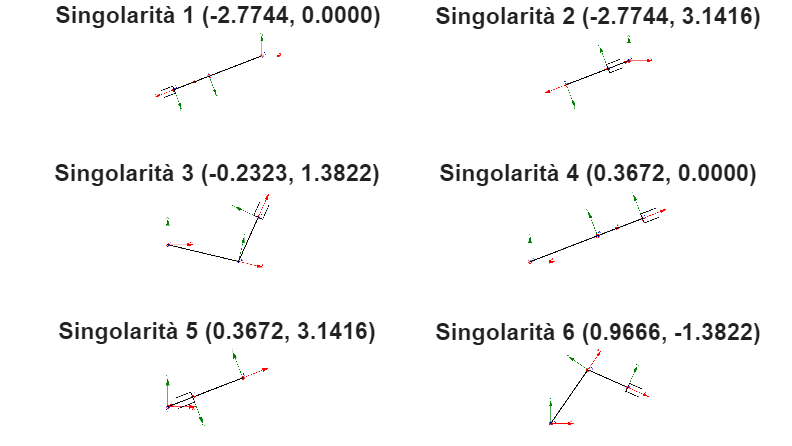
\includegraphics[width=1\linewidth]{figure_0.png}
\end{center}

\begin{par}
\begin{flushleft}
Per comprendere visivamente il comportamento degli algoritmi di ottimizzazione, è essenziale visualizzare il la funzione di costo $V(q)$. Questo viene fatto generando una superficie 3D della funzione nello spazio dei giunti $(q_1 ,q_2 )$. Su questo grafico, verranno sovrapposti i punti critici calcolati e classificati. Questo permette di vedere dove si trovano i minimi, i massimi e i punti di sella, che possono deviare o intrappolare gli algoritmi.
\end{flushleft}
\end{par}
\newpage
\begin{matlabcode}
l_val = [1, 0.8];
for i = 1:size(puntiCritici, 1)
    q1Crit = puntiCritici(i,1);
    q2Crit = puntiCritici(i,2);
    l1Crit = l_val(1);
    l2Crit = l_val(2);
    fprintf('Configurazione Critica (q1, q2) = (%.4f, %.4f)\n', q1Crit, q2Crit);

    % Posizione Base Giunto
    x0 = 0;
    y0 = 0;

    % Calcolo Coordinate Fine Primo Braccio (x1, y1)
    x1Crit = double(l1Crit * cos(q1Crit));
    y1Crit = double(l1Crit * sin(q1Crit));

    % Calcolo Coordinate End Effector (x2, y2) Rispetto Al Sistema Di Riferimento Base
    x2Crit = double(x1Crit + l2Crit * cos(q1Crit + q2Crit));
    y2Crit = double(y1Crit + l2Crit * sin(q1Crit + q2Crit));

    fprintf('\t Posizione Giunto 0 (Base) (x0, y0) = (%.4f, %.4f)\n', x0, y0);
    fprintf('\t Posizione Giunto 1        (x1, y1) = (%.4f, %.4f)\n', x1Crit, y1Crit);
    fprintf('\t Posizione Giunto 2 (EE)   (x2, y2) = (%.4f, %.4f)\n', x2Crit, y2Crit);

end
\end{matlabcode}
\begin{matlaboutput}
Configurazione Critica (q1, q2) = (-2.7744, 0.0000)
	 Posizione Giunto 0 (Base) (x0, y0) = (0.0000, 0.0000)
	 Posizione Giunto 1        (x1, y1) = (-0.9333, -0.3590)
	 Posizione Giunto 2 (EE)   (x2, y2) = (-1.6800, -0.6462)
Configurazione Critica (q1, q2) = (-2.7744, 3.1416)
	 Posizione Giunto 0 (Base) (x0, y0) = (0.0000, 0.0000)
	 Posizione Giunto 1        (x1, y1) = (-0.9333, -0.3590)
	 Posizione Giunto 2 (EE)   (x2, y2) = (-0.1867, -0.0718)
Configurazione Critica (q1, q2) = (-0.2323, 1.3822)
	 Posizione Giunto 0 (Base) (x0, y0) = (0.0000, 0.0000)
	 Posizione Giunto 1        (x1, y1) = (0.9731, -0.2302)
	 Posizione Giunto 2 (EE)   (x2, y2) = (1.3000, 0.5000)
Configurazione Critica (q1, q2) = (0.3672, 0.0000)
	 Posizione Giunto 0 (Base) (x0, y0) = (0.0000, 0.0000)
	 Posizione Giunto 1        (x1, y1) = (0.9333, 0.3590)
	 Posizione Giunto 2 (EE)   (x2, y2) = (1.6800, 0.6462)
Configurazione Critica (q1, q2) = (0.3672, 3.1416)
	 Posizione Giunto 0 (Base) (x0, y0) = (0.0000, 0.0000)
	 Posizione Giunto 1        (x1, y1) = (0.9333, 0.3590)
	 Posizione Giunto 2 (EE)   (x2, y2) = (0.1867, 0.0718)
Configurazione Critica (q1, q2) = (0.9666, -1.3822)
	 Posizione Giunto 0 (Base) (x0, y0) = (0.0000, 0.0000)
	 Posizione Giunto 1        (x1, y1) = (0.5681, 0.8230)
	 Posizione Giunto 2 (EE)   (x2, y2) = (1.3000, 0.5000)
\end{matlaboutput}

\newpage
\begin{matlabcode}
%% Visualizzazione Funzione di Costo V(q) e Punti Critici

% Definizione Dominio
q1_range = linspace(-pi, pi, 150);
q2_range = linspace(-pi, pi, 150);

% Creazione Griglia
[Q1, Q2] = meshgrid(q1_range, q2_range);

% Inizializzazione Matrice
V_grid = zeros(size(Q1));

% Calcolare V(q) Su Ogni Punto

% fprintf('Calcolo della superficie di costo V(q)... (potrebbe richiedere tempo)\n');
for i = 1:length(q1_range)
    for j = 1:length(q2_range)
        q1_current = Q1(i, j);
        q2_current = Q2(i, j);
        V_grid(i, j) = subs(V_val, [q1, q2], [q1_current, q2_current]);
    end
end


% Generare Grafico
figure('Name', 'Funzione Di Costo');
contourf(Q1, Q2, V_grid, 20);

title('Funzione di Costo V(q) e Punti Critici');
xlabel('q_1 [rad]');
ylabel('q_2 [rad]');
colorbar;
axis equal;
axis tight;
hold on;

% Iterarezione Sui Punti Critici
e_q_val = subs(e_q, [l1, l2, rx, ry], [l_val(1), l_val(2), r_val(1), r_val(2)]);

for i = 1:size(puntiCritici, 1)
    qCrit = puntiCritici(i, :);

    H_V_Current = double(subs(H_V_val, [q1, q2], qCrit));
    lambda = eig(H_V_Current);

    e_current_norm = norm(double(subs(e_q_val, [q1, q2], qCrit)));

    if all(lambda > 0)
        if e_current_norm < 1e-5
            % Pentagramma Verde ('gp')
            plot(qCrit(1), qCrit(2), 'gp', 'MarkerSize', 15, 'MarkerFaceColor', 'g', 'LineWidth', 2);
        else
            plot(qCrit(1), qCrit(2), 'go', 'MarkerSize', 12, 'MarkerFaceColor', 'g');
        end
\end{matlabcode}
\newpage
\begin{matlabcode}
    elseif all(lambda < 0)
        % Quadrato Rosso ('rs')
        plot(qCrit(1), qCrit(2), 'rs', 'MarkerSize', 12, 'MarkerFaceColor', 'r');
    else % Punto di Sella
        % Croce Blu ('bx')
        plot(qCrit(1), qCrit(2), 'bx', 'MarkerSize', 15, 'LineWidth', 2.5);
    end
end

% Legenda
h_min_g = plot(NaN, NaN, 'gp', 'MarkerSize', 15, 'MarkerFaceColor', 'g', 'LineWidth', 2);
h_max_l = plot(NaN, NaN, 'rs', 'MarkerSize', 12, 'MarkerFaceColor', 'r');
h_sella = plot(NaN, NaN, 'bx', 'MarkerSize', 15, 'LineWidth', 2.5);

legend([h_min_g, h_max_l, h_sella], ...
       'Minimo Globale', 'Massimo Locale', 'Punto di Sella', ...
       'Location', 'best');

hold off;
\end{matlabcode}
\begin{center}
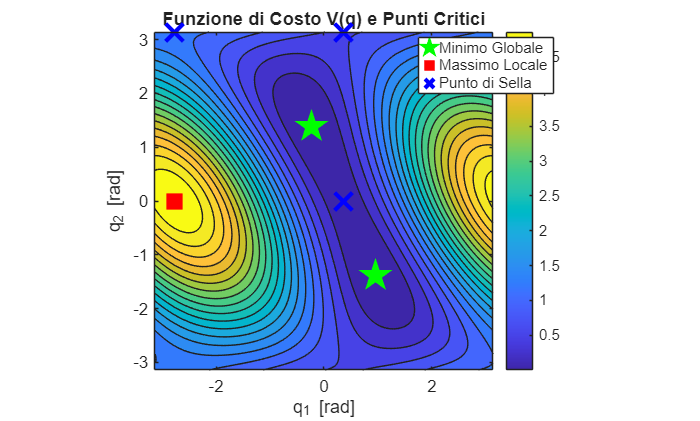
\includegraphics[width=1\linewidth]{figure_1.png}
\end{center}


\newpage
\matlabheadingtwo{Algoritmo Newton Iterativo}

\begin{matlabcode}
fprintf('----- Algoritmo Di Newton Iterativo -----');
\end{matlabcode}
\begin{matlaboutput}
----- Algoritmo Di Newton Iterativo -----
\end{matlaboutput}
\begin{matlabcode}
% Valori N Bracci
l1_val = 1.0;
l2_val = 1.0;

% Posa Desiderata
r_val = [1.0; 1.0];

% Parametri Robot
T = 0.1;
k_gain = 5;
K_num = k_gain * eye(2);

% Creazione Funzioni Simboliche
fr_fun = matlabFunction(fr_q, 'Vars', {l1, l2, q1, q2});
J_fun = matlabFunction(J_q, 'Vars', {l1, l2, q1, q2});

% Condizioni Iniziali
q_initial_conditions = [
    pi/4, pi/4;      % Configurazione iniziale 1
    0, pi/2;         % Configurazione iniziale 2
    -pi/3, pi/6      % Configurazione iniziale 3
];

nrSol = size(q_initial_conditions, 1);

for i = 1:nrSol
    q_k = q_initial_conditions(i, :).'; % Vettore Colonna

    fprintf('Test %d: Condizione Iniziale q0 = [%.4f, %.4f]\n', i, q_k(1), q_k(2));

    % Inizializzazione Array Cronologia
    q_history = zeros(2, 100 + 1);
    error_history = zeros(1, 100);
    q_history(:, 1) = q_k;

    for k = 1:100
        pos_k = fr_fun(l1_val, l2_val, q_k(1), q_k(2));

        e_k = r_val - pos_k;
        error_norm = norm(e_k);
        error_history(k) = error_norm;

        if error_norm < 1e-6
            fprintf('\t Convergenza Raggiunta In %d Iterazioni.\n', k);
            break;
        end

        J_k = J_fun(l1_val, l2_val, q_k(1), q_k(2));

        if abs(det(J_k)) < 1e-5
            fprintf('\t Attenzione: Jacobiano Quasi Singolare (det(J) = %.2e). Interruzione.\n', det(J_k));
            break;
        end

        % f. Aggiornamento Configurazione Giunti (Formula di Newton)
        % q_{k+1} = q_k + T * J^{-1}(q_k) * K * e(k)
        q_k = q_k + T * inv(J_k) * K_num * e_k;

        % Salvataggio Nuova Configurazione
        q_history(:, k+1) = q_k;
    end

    if k == 100 && error_norm >= 1e-6
        fprintf('\t Algoritmo Terminato Per Numero Massimo Iterazioni.\n');
    end

    % Tronca Cronoplogia Al Numero Di Iterazioni Effettive
    q_history = q_history(:, 1:k);

    % Visualizzazione Risultati
    q_finale = q_history(:, end);
    pos_finale = fr_fun(l1_val, l2_val, q_finale(1), q_finale(2));

    fprintf('\t Configurazione finale q_f: [%.4f, %.4f]\n', q_finale(1), q_finale(2));
    fprintf('\t Posizione finale EE [x; y]: [%.4f; %.4f]\n', pos_finale(1), pos_finale(2));
    fprintf('\t Errore finale (norma): %.2e\n', norm(r_val - pos_finale));
end
\end{matlabcode}
\begin{matlaboutput}
Test 1: Condizione Iniziale q0 = [0.7854, 0.7854]
	 Convergenza Raggiunta In 21 Iterazioni.
	 Configurazione finale q_f: [0.0000, 1.5708]
	 Posizione finale EE [x; y]: [1.0000; 1.0000]
	 Errore finale (norma): 6.98e-07
Test 2: Condizione Iniziale q0 = [0.0000, 1.5708]
	 Convergenza Raggiunta In 1 Iterazioni.
	 Configurazione finale q_f: [0.0000, 1.5708]
	 Posizione finale EE [x; y]: [1.0000; 1.0000]
	 Errore finale (norma): 0.00e+00
Test 3: Condizione Iniziale q0 = [-1.0472, 0.5236]
	 Convergenza Raggiunta In 27 Iterazioni.
	 Configurazione finale q_f: [-4.7124, 4.7124]
	 Posizione finale EE [x; y]: [1.0000; 1.0000]
	 Errore finale (norma): 6.88e-07
\end{matlaboutput}

\newpage
\matlabheadingtwo{Algoritmo Gradiente Iterativo}

\begin{matlabcode}
fprintf('----- Algoritmo Gradiente Iterativo -----');
\end{matlabcode}
\begin{matlaboutput}
----- Algoritmo Gradiente Iterativo -----
\end{matlaboutput}
\begin{matlabcode}
% Learning Rate
alpha_val = 0.8;

for i = 1:nrSol
    q_k = q_initial_conditions(i, :).'; % Vettore Colonna

    fprintf('\nTest %d: Condizione Iniziale q0 = [%.4f, %.4f]\n', i, q_k(1), q_k(2));

    % Inizializzazione Array Cronologia
    q_history_grad = zeros(2, 500 + 1);
    error_history_grad = zeros(1, 500);
    q_history_grad(:, 1) = q_k;

    iter_effettive = 500;

    for k = 1:500
        % Calcolo Posizione Corrente EE
        pos_k = fr_fun(l1_val, l2_val, q_k(1), q_k(2));

        % Calcolo Errore Corrente
        e_k = r_val - pos_k;
        error_norm = norm(e_k);
        error_history_grad(k) = error_norm;

        % Condizione di Arresto per Convergenza
        if error_norm < 1e-6
            fprintf('\t Convergenza Raggiunta In %d Iterazioni.\n', k);
            iter_effettive = k;
            break;
        end

        % Calcolo Jacobiano alla Configurazione Corrente
        J_k = J_fun(l1_val, l2_val, q_k(1), q_k(2));

        % Robustezza alle Singolarità
        % La trasposta J_k.' esiste sempre, quindi l'algoritmo non fallisce numericamente ma
        % rallenta la convergenza fino a fermarsi se si trova esattamente su un minimo locale.

        % Aggiornamento Configurazione Giunti (Formula del Gradiente)
        % q_{k+1} = q_k + T * alpha * J(q_k)^T * e(k)
        q_k = q_k + T * alpha_val * J_k.' * e_k;

        % Salvataggio Nuova Configurazione
        q_history_grad(:, k+1) = q_k;
    end

    if k == 500 && error_norm >= 1e-6
        fprintf('\t Algoritmo Terminato Per Numero Massimo Iterazioni.\n');
    end
\end{matlabcode}
\newpage
\begin{matlabcode}
    % Tronca Cronologia Al Numero Di Iterazioni Effettive
    q_history_grad = q_history_grad(:, 1:iter_effettive);

    % Visualizzazione Risultati
    q_finale_grad = q_history_grad(:, end);
    pos_finale_grad = fr_fun(l1_val, l2_val, q_finale_grad(1), q_finale_grad(2));

    fprintf('\t Configurazione Finale q_f: [%.4f, %.4f]\n', q_finale_grad(1), q_finale_grad(2));
    fprintf('\t Posizione Finale EE [x; y]: [%.4f; %.4f]\n', pos_finale_grad(1), pos_finale_grad(2));
    fprintf('\t Errore Finale (norma): %.2e\n', norm(r_val - pos_finale_grad));
end
\end{matlabcode}
\begin{matlaboutput}
Test 1: Condizione Iniziale q0 = [0.7854, 0.7854]
	 Convergenza Raggiunta In 468 Iterazioni.
	 Configurazione Finale q_f: [0.0000, 1.5708]
	 Posizione Finale EE [x; y]: [1.0000; 1.0000]
	 Errore Finale (norma): 9.75e-07
Test 2: Condizione Iniziale q0 = [0.0000, 1.5708]
	 Convergenza Raggiunta In 1 Iterazioni.
	 Configurazione Finale q_f: [0.0000, 1.5708]
	 Posizione Finale EE [x; y]: [1.0000; 1.0000]
	 Errore Finale (norma): 0.00e+00
Test 3: Condizione Iniziale q0 = [-1.0472, 0.5236]
	 Convergenza Raggiunta In 403 Iterazioni.
	 Configurazione Finale q_f: [0.0000, 1.5708]
	 Posizione Finale EE [x; y]: [1.0000; 1.0000]
	 Errore Finale (norma): 9.91e-07
\end{matlaboutput}

\end{document}
